\documentclass[journal,12pt,twocolumn]{IEEEtran}
\usepackage{amsthm}
\allowbreak
\usepackage{setspace}
\usepackage{gensymb}
\singlespacing
\usepackage[cmex10]{amsmath}
\usepackage{caption}
\usepackage{amsthm}



\DeclareUnicodeCharacter{2212}{-}
\usepackage{tikz}
\usepackage{pgfplots}
\usepackage{tkz-fct}
\usepackage{mathrsfs}
\usepackage{txfonts}
\usepackage{stfloats}
\usepackage{bm}
\usepackage{cite}
\usepackage{cases}
\usepackage{subfig}

\usepackage{longtable}
\usepackage{multirow}

\usepackage{enumitem}
\usepackage{mathtools}
\usepackage{steinmetz}
\usepackage{tikz}
\usepackage{circuitikz}
\usepackage{verbatim}
\usepackage{tfrupee}
\usepackage[breaklinks=true]{hyperref}
\usepackage{graphicx}
\usepackage{tkz-euclide}
\graphicspath{ {./images/} }
\usetikzlibrary{calc,math}
\usepackage{listings}
    \usepackage{color}                                            %%
    \usepackage{array}                                            %%
    \usepackage{longtable}                                        %%
    \usepackage{calc}                                             %%
    \usepackage{multirow}                                         %%
    \usepackage{hhline}                                           %%
    \usepackage{ifthen}                                           %%
    \usepackage{lscape}     
\usepackage{multicol}
\usepackage{chngcntr}

\DeclareMathOperator*{\Res}{Res}

\renewcommand\thesection{\arabic{section}}
\renewcommand\thesubsection{\thesection.\arabic{subsection}}
\renewcommand\thesubsubsection{\thesubsection.\arabic{subsubsection}}

\renewcommand\thesectiondis{\arabic{section}}
\renewcommand\thesubsectiondis{\thesectiondis.\arabic{subsection}}
\renewcommand\thesubsubsectiondis{\thesubsectiondis.\arabic{subsubsection}}


\hyphenation{op-tical net-works semi-conduc-tor}
\def\inputGnumericTable{}                                 %%

\lstset{
%language=C,
frame=single, 
breaklines=true,
columns=fullflexible
}
\begin{document}


\newtheorem{theorem}{Theorem}[section]
\newtheorem{problem}{Problem}
\newtheorem{proposition}{Proposition}[section]
\newtheorem{lemma}{Lemma}[section]
\newtheorem{corollary}[theorem]{Corollary}
\newtheorem{example}{Example}[section]
\newtheorem{definition}[problem]{Definition}

\newcommand{\BEQA}{\begin{eqnarray}}
\newcommand{\EEQA}{\end{eqnarray}}
\newcommand{\define}{\stackrel{\triangle}{=}}
\bibliographystyle{IEEEtran}
\raggedbottom
\setlength{\parindent}{0pt}
\providecommand{\mbf}{\mathbf}
\providecommand{\pr}[1]{\ensuremath{\Pr\left(#1\right)}}
\providecommand{\qfunc}[1]{\ensuremath{Q\left(#1\right)}}
\providecommand{\sbrak}[1]{\ensuremath{{}\left[#1\right]}}
\providecommand{\lsbrak}[1]{\ensuremath{{}\left[#1\right.}}
\providecommand{\rsbrak}[1]{\ensuremath{{}\left.#1\right]}}
\providecommand{\brak}[1]{\ensuremath{\left(#1\right)}}
\providecommand{\lbrak}[1]{\ensuremath{\left(#1\right.}}
\providecommand{\rbrak}[1]{\ensuremath{\left.#1\right)}}
\providecommand{\cbrak}[1]{\ensuremath{\left\{#1\right\}}}
\providecommand{\lcbrak}[1]{\ensuremath{\left\{#1\right.}}
\providecommand{\rcbrak}[1]{\ensuremath{\left.#1\right\}}}
\theoremstyle{remark}
\newtheorem{rem}{Remark}
\newcommand{\sgn}{\mathop{\mathrm{sgn}}}
\providecommand{\abs}[1]{$\left\vert#1\right\vert$}
\providecommand{\res}[1]{\Res\displaylimits_{#1}} 
\providecommand{\norm}[1]{$\left\lVert#1\right\rVert$}
%\providecommand{\norm}[1]{\lVert#1\rVert}
\providecommand{\mtx}[1]{\mathbf{#1}}
\providecommand{\mean}[1]{E$\left[ #1 \right]$}
\providecommand{\fourier}{\overset{\mathcal{F}}{ \rightleftharpoons}}
%\providecommand{\hilbert}{\overset{\mathcal{H}}{ \rightleftharpoons}}
\providecommand{\system}{\overset{\mathcal{H}}{ \longleftrightarrow}}
	%\newcommand{\solution}[2]{\textbf{Solution:}{#1}}
\newcommand{\solution}{\noindent \textbf{Solution: }}
\newcommand{\cosec}{\,\text{cosec}\,}
\providecommand{\dec}[2]{\ensuremath{\overset{#1}{\underset{#2}{\gtrless}}}}
\newcommand{\myvec}[1]{\ensuremath{\begin{pmatrix}#1\end{pmatrix}}}
\newcommand{\mydet}[1]{\ensuremath{\begin{vmatrix}#1\end{vmatrix}}}
\numberwithin{equation}{subsection}
\makeatletter
\@addtoreset{figure}{problem}
\makeatother
\let\StandardTheFigure\thefigure
\let\vec\mathbf
\renewcommand{\thefigure}{\theproblem}
\def\putbox#1#2#3{\makebox[0in][l]{\makebox[#1][l]{}\raisebox{\baselineskip}[0in][0in]{\raisebox{#2}[0in][0in]{#3}}}}
     \def\rightbox#1{\makebox[0in][r]{#1}}
     \def\centbox#1{\makebox[0in]{#1}}
     \def\topbox#1{\raisebox{-\baselineskip}[0in][0in]{#1}}
     \def\midbox#1{\raisebox{-0.5\baselineskip}[0in][0in]{#1}}
\vspace{3cm}
\title{AI1103: Assignment 9}
\author{Tanmay Garg \\CS20BTECH11063 EE20BTECH11048}
\maketitle
\newpage
\bigskip
\renewcommand{\thefigure}{\theenumi}
\renewcommand{\thetable}{\theenumi}
%
Download latex-tikz codes from 
%
\begin{lstlisting}
https://github.com/tanmaygar/AI-Course/blob/main/Assignment9/Assignment9.tex
\end{lstlisting}
\section*{Problem CSIR UGC NET EXAM (June 2016), Q.118: }
Three types of components are used in electrical circuits 1, 2, 3 as shown below in the figure
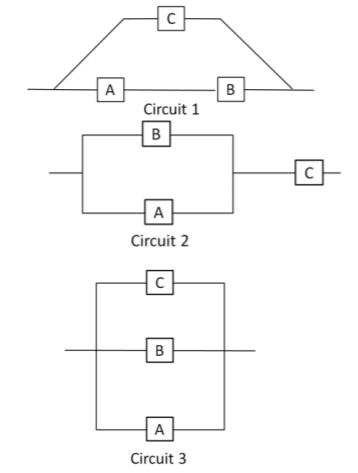
\includegraphics[width=\columnwidth]{circuits.png}
Suppose that each of the three components fail with probability $p$ and independently of each other. Let $q_i = \pr{\text{Circuit $i$ does not fail}}$; $i=1,2,3$ For $0<p<1$, we have
\begin{multicols}{2}
    \begin{enumerate}
        \item $q_3>q_1$
        \item $q_2=q_1$
        \item $q_2>q_1$
        \item $q_2>q_3$
    \end{enumerate}
\end{multicols}

\section*{Solution:}

%In the Truth Table:
%\begin{table}[]
%    \centering
%    \begin{tabular}{|c|c|}
%    \hline
%        1 & Element works \\
%        0 & Element fails\\
%         \hline
%    \end{tabular}
%    \caption{Value}
%    \label{tab:truth}
%\end{table}

For $q_1$, the truth table\\

\begin{table}[h]
    \centering
    \begin{tabular}{|c|c|c|c|}
    \hline
         $A$ & $B$ & $C$ & $(A \land B) \lor C$ \\
         \hline
         1 &1  & 0 &1\\\hline
         1&1&1&1\\\hline
         0&1&1&1\\\hline
         0&0&1&1\\\hline
         1&0&1&1\\
    \hline
    \end{tabular}
    \caption{Circuit 1 working}
    \label{tab:my_label}
\end{table}

Multiplying and adding probability for each case of $q_1$gives
\begin{align}
    q_1 = p^3-2p^2+1
\end{align}
For $q_2$,
\begin{table}[h]
    \centering
    \begin{tabular}{|c|c|c|c|}
    \hline
         $A$ & $B$ & $C$ & $(A \lor B) \land C$ \\
         \hline
         1&1&1&1\\ \hline
         1&0&1&1\\\hline
         0&1&1&1\\
    \hline
    \end{tabular}
    \caption{Circuit 2 working}
    \label{tab:table2}
\end{table}

Multiplying and adding probability for each case of $q_2$ gives
\begin{align}
    q_2 = p^3-p^2-p+1
\end{align}

For $q_3$, the truth table
\begin{table}[h]
    \centering
    \begin{tabular}{|c|c|c|c|}
    \hline
         $A$ & $B$ & $C$ & $A \lor B \lor C$ \\
         \hline
         1&0&0&1\\\hline
         0&1&0&1\\\hline
         0&0&1&1\\\hline
         1&1&0&1\\\hline
         1&0&1&1\\\hline
         0&1&1&1\\\hline
         1&1&1&1\\
    \hline
    \end{tabular}
    \caption{Circuit 3 working}
    \label{tab:table3}
\end{table}

Multiplying and adding probability for each case of $q_3$ gives
\begin{align}
    q_3 = 1-p^3
\end{align}
%%
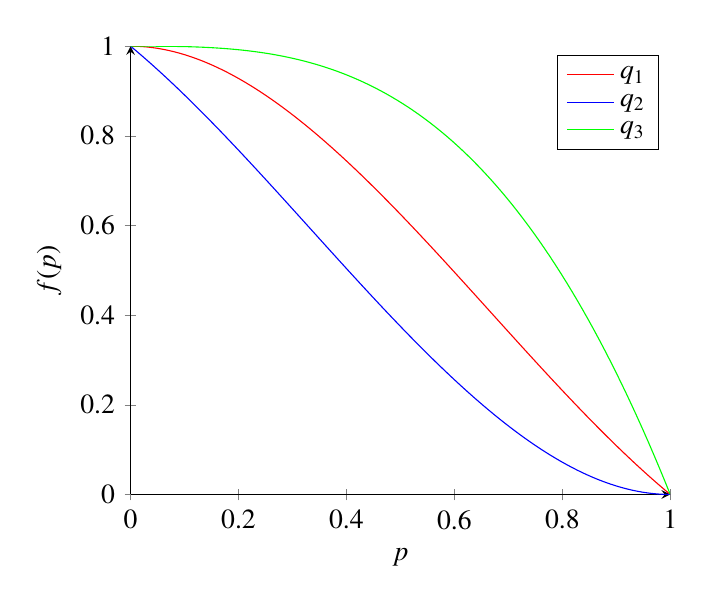
\begin{tikzpicture}
\begin{axis}[
    axis lines = left,
    xlabel = $p$,
    ylabel = {$f(p)$},
]

\addplot [
    domain=0:1, 
    samples=100, 
    color=red,
]
{x^3-2*x^2+1};
\addlegendentry{$q_1$}

\addplot [
    domain=0:1, 
    samples=100, 
    color=blue,
    ]
    {x^3-x^2-x+1};
\addlegendentry{$q_2$}
\addplot [
    domain=0:1, 
    samples=100, 
    color=green,
]
{1-x^3};
\addlegendentry{$q_3$}
\end{axis}
\end{tikzpicture}
\begin{align}
    \therefore q_3>q_1>q_2
\end{align}
Hence \textbf{Option 1} is correct
\end{document}